% -*- mode: latex; -*- mustache tags:  
\documentclass[10pt,twoside,english]{_support/latex/sbabook/sbabook}
\let\wholebook=\relax

\usepackage{import}
\subimport{_support/latex/}{common.tex}

%=================================================================
% Debug packages for page layout and overfull lines
% Remove the showtrims document option before printing
\ifshowtrims
  \usepackage{showframe}
  \usepackage[color=magenta,width=5mm]{_support/latex/overcolored}
\fi


% =================================================================
\title{Learning Object-Oriented Programming, Design and TDD with Pharo}
\author{Stéphane Ducasse}
\series{The Pharo TextBook Collection}

\hypersetup{
  pdftitle = {Learning Object-Oriented Programming, Design and TDD with Pharo},
  pdfauthor = {Stéphane Ducasse},
  pdfkeywords = {Introduction, programming, design, testing, Pharo, Smalltalk}
}


% =================================================================
\begin{document}

% Title page and colophon on verso
\maketitle
\pagestyle{titlingpage}
\thispagestyle{titlingpage} % \pagestyle does not work on the first one…

\cleartoverso
{\small

  Copyright 2017 by Stéphane Ducasse.

  The contents of this book are protected under the Creative Commons
  Attribution-ShareAlike 3.0 Unported license.

  You are \textbf{free}:
  \begin{itemize}
  \item to \textbf{Share}: to copy, distribute and transmit the work,
  \item to \textbf{Remix}: to adapt the work,
  \end{itemize}

  Under the following conditions:
  \begin{description}
  \item[Attribution.] You must attribute the work in the manner specified by the
    author or licensor (but not in any way that suggests that they endorse you
    or your use of the work).
  \item[Share Alike.] If you alter, transform, or build upon this work, you may
    distribute the resulting work only under the same, similar or a compatible
    license.
  \end{description}

  For any reuse or distribution, you must make clear to others the
  license terms of this work. The best way to do this is with a link to
  this web page: \\
  \url{http://creativecommons.org/licenses/by-sa/3.0/}

  Any of the above conditions can be waived if you get permission from
  the copyright holder. Nothing in this license impairs or restricts the
  author's moral rights.

  \begin{center}
    
\includegraphics[width=0.2\textwidth]{_support/latex/sbabook/CreativeCommons-BY-SA.pdf}
  \end{center}

  Your fair dealing and other rights are in no way affected by the
  above. This is a human-readable summary of the Legal Code (the full
  license): \\
  \url{http://creativecommons.org/licenses/by-sa/3.0/legalcode}

  \vfill

  % Publication info would go here (publisher, ISBN, cover design…)
  Layout and typography based on the \textcode{sbabook} \LaTeX{} class by Damien
  Pollet.
}


\frontmatter
\pagestyle{plain}

\tableofcontents*
\clearpage\listoffigures

\mainmatter

\chapter{Stone Paper Scissors}\label{cha_stone}
As we already saw sending a message is in fact making a choice. Indeed when we send a message, the method associated with the method in the class hierarchy of the receiver will be selected and executed. 

Now we often have cases where we would like to select a method based on the receiver of the message and one argument. 
Again there is a simple solution named double dispatch that consists in sending another message to the argument hence making two choices one after the other. 

This technique while simple can be challenging to grasp because programmers are so used to think that choices are made using explicit conditionals.  In this chapter we will show an example of double dispatch via the paper stone scissors game. 
\section{Starting with a couple of tests}
\begin{displaycode}{plain}
TestCase subclass: #StonePaperScissorsTest
	instanceVariableNames: ''
	classVariableNames: ''
	package: 'StonePaperScissors'
\end{displaycode}

\begin{displaycode}{plain}
StonePaperScissorsTest >> testPaperIsWinning
	self assert: (Stone new play: Paper new) = #paper
\end{displaycode}

\begin{displaycode}{plain}
StonePaperScissorsTest >> testScissorIsWinning
	self assert: (Scissors new play: Paper new) = #scissors
\end{displaycode}

\begin{displaycode}{plain}
StonePaperScissorsTest >> testStoneAgainsStone
	self assert: (Stone new play: Stone new) = #draw
\end{displaycode}
\section{Creating the classes}
\begin{displaycode}{plain}
Object subclass: #Paper
	instanceVariableNames: ''
	classVariableNames: ''
	package: 'StonePaperScissors'
\end{displaycode}

\begin{displaycode}{plain}
Object subclass: #Scissors
	instanceVariableNames: ''
	classVariableNames: ''
	package: 'StonePaperScissors'
\end{displaycode}

\begin{displaycode}{plain}
Object subclass: #Stone
	instanceVariableNames: ''
	classVariableNames: ''
	package: 'StonePaperScissors'
\end{displaycode}

They could share a common superclass
\section{With messages}
\begin{displaycode}{plain}
StonePaperScissorsTest >> testPaperIsWinning
	self assert: (Stone new play: Paper new) = #paper
\end{displaycode}

\begin{displaycode}{plain}
Stone >> play: anotherTool
	^ anotherTool playAgainstStone: self
\end{displaycode}

\begin{displaycode}{plain}
Paper >> playAgainstStone: aStone
	^ #paper
\end{displaycode}

The test should pass now. 
\subsection{playAgainstStone:}
\begin{displaycode}{plain}
Scissors >> playAgainstStone: aStone
	^ #stone
\end{displaycode}

\begin{displaycode}{plain}
Stone >> playAgainstStone: aStone
	^ #draw
\end{displaycode}
\subsection{Scissors now}
\begin{displaycode}{plain}
StonePaperScissorsTest >> testScissorIsWinning
	self assert: (Scissors new play: Paper new) = #scissors
\end{displaycode}

\begin{displaycode}{plain}
Scissors >> play: anotherTool
	^ anotherTool playAgainstScissors: self
\end{displaycode}

\begin{displaycode}{plain}
Scissors >> playAgainstScissors: aScissors
	^ #draw
\end{displaycode}

\begin{displaycode}{plain}
Paper >> playAgainstScissors: aScissors
	^ #scissors
\end{displaycode}

\begin{displaycode}{plain}
Stone >> playAgainstScissors: aScissors
	^ #stone
\end{displaycode}
\subsection{Paper now}
\begin{displaycode}{plain}
Paper >> play: anotherTool
	^ anotherTool playAgainstPaper: self
\end{displaycode}

\begin{displaycode}{plain}
Scissors >> playAgainstPaper: aPaper
	^ #scissors
\end{displaycode}

\begin{displaycode}{plain}
Paper >> playAgainstPaper: aPaper
	^ #draw
\end{displaycode}

\begin{displaycode}{plain}
Stone >> playAgainstPaper: aPaper
	^ #paper
\end{displaycode}


\begin{figure}

\begin{center}
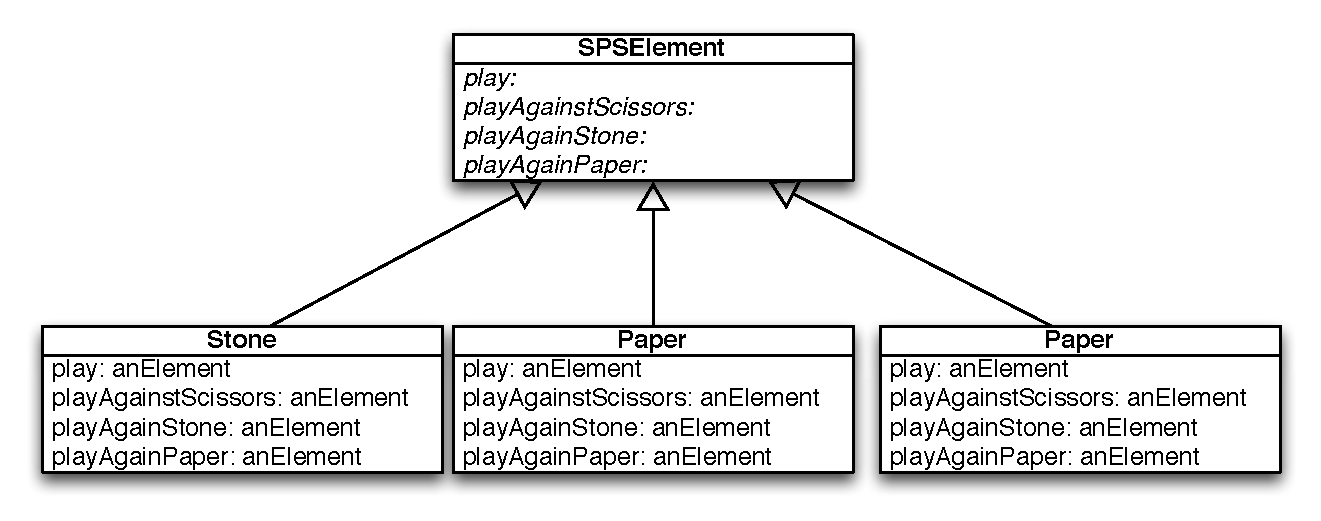
\includegraphics[width=0.8\textwidth]{/Users/ducasse/Workspace/FirstCircle/MyBooks/Bk-Writing/PharoBooks/LearningOOPWithPharoTrans/_result/pdf/Chapters/PaperStoneScissor/figures/StonePaperScissors.pdf}\caption{An overview of a possible solution using double dispatch.\label{/Users/ducasse/Workspace/FirstCircle/MyBooks/Bk-Writing/PharoBooks/LearningOOPWithPharoTrans/_result/pdf/Chapters/PaperStoneScissor/figures/StonePaperScissors.pdf}}\end{center}
\end{figure}


The methods could return a value such as 1 when the receiver wins, 0 when there is draw and -1 when the receiver loses.  Add new tests and check this version. 
\section{A Better API}
Both previous approaches either returning a symbol or a number are working but we can ask ourselves how the client will use this code. 

Most of the time he will have to check again the returned result to perform some actions.

\begin{displaycode}{plain}
(aGameElement play: anotherGameElement) = 1 
	ifTrue: [ do something for aGameElement]
	(aGameElement play: anotherGameElement) = -1 
\end{displaycode}

So all in all, while this was a good exercise to help you understand that we do not need to have explicit conditionals and that we can use message passing instead, it felt a bit disappointing. 

But there is a much better solution using double dispatch. The idea is to pass the action to be executed to the object and that the object decide what to do. 

\begin{displaycode}{plain}
Paper new competeWith: Paper new
	onDraw: [ Game incrementDraw ]
	onReceiverWin: [ ]
	onReceiverLose: [ ]
\end{displaycode}

\begin{displaycode}{plain}
Paper new competeWith: Stone new
	onDraw: [ ]
	onReceiverWin: [ Game incrementPaper ]
	onReceiverLose: [ ]
\end{displaycode}

Propose an implementation.
\section{A possible implementation}
\begin{displaycode}{plain}
Paper >> play: anElement onDraw: aDrawBlock onWin: aWinBlock onLose: aLoseBlock
	^ anElement
		playAgainstPaper: self
		onDraw: aDrawBlock
		onReceiverWin: aWinBlock
		onReceiverLose: aLoseBlock
\end{displaycode}

\begin{displaycode}{plain}
Paper >> playAgainstPaper: anElement onDraw: aDrawBlock onReceiverWin: aWinBlock onReceiverLose: aLoseBlock
	^ aDrawBlock value
\end{displaycode}
\section{Conclusion}
Sending a message is making a choice amongst several methods. Depending on the receiver of a message the correct method will be selected. Therefore sending a message is making a choice and the different classes represent the possible alternatives. 

Now this example illustrates this point but going even further. Here we wanted to be able to make a choice depending on both an object and the argument of the message. The solution shows that it is enough to send back another message 
to the argument to perform a second selection that because of the first message now realizes a choice based on a message receiver and its argument. 


% lulu requires an empty page at the end. That's why I'm using
% \backmatter here.
\backmatter

% Index would go here
\bibliographystyle{abbrv}
\bibliography{others.bib}
\end{document}
